\documentclass[12pt]{extarticle}
\usepackage[utf8]{inputenc}
\usepackage{verbatim}
\usepackage{enumitem}
\usepackage{cite}
\usepackage{graphicx}
\usepackage{wrapfig}
\PassOptionsToPackage{hyphens}{url}\usepackage{hyperref}

\title{EE212 \\ Homework 2 --  555 Timer}
\author{Mehdi Saffar -- 2016400411}
\date{May 2019}

\begin{document}
\maketitle
\section{What is the 555 timer?}
The 555 timer is a very useful electronic component that is used in almost all circuits that require some sort of time control. It was designed by Hans Camenzing and introduced in 1971 by the American company Signetics. It is so popular that a billion units were manufactured back in 2003 alone. Its name comes from the fact that it internally uses three 5k$\Omega$ resistors to generate two reference voltages in a voltage divider setting.

\section{What does it look like?}
\begin{center}
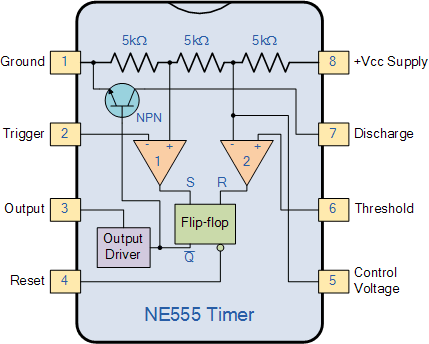
\includegraphics[width=8cm]{form.png}
\end{center}
Internally, it is constituted of a voltage divider current (the three resistors), two comparators, a flip-flop and a high current output stage. It is made of about 25 transistors, 2 diodes and 16 resistors in total. It comes in a bipolar 8-pin DIP package.

The pin specification is as follows:
\begin{center}
\begin{tabular}{|c|c|p{10cm}|}
\hline
\textbf{\#} & \textbf{Name} & \textbf{Description}\\
\hline
1 & Ground & Ground reference voltage, low level (0 V)\\
\hline
2 & Trigger & The OUT pin goes high and a timing interval starts when this input falls below 1/2 of CTRL voltage (which is typically 1/3 Vcc, CTRL being 2/3 Vcc by default if CTRL is left open). In other words, OUT is high as long as the trigger low. Output of the timer totally depends upon the amplitude of the external trigger voltage applied to this pin.\\
\hline
3 & Output & This output is driven to approximately 1.7 V below +Vcc, or to GND.\\
\hline
4 & Reset & A timing interval may be reset by driving this input to GND, but the timing does not begin again until RESET rises above approximately 0.7 volts. Overrides TRIG which overrides threshold.\\
\hline
5 & Control & Provides “control” access to the internal voltage divider (by default, 2/3 Vcc).\\
\hline
6 & Threshold & The timing (OUT high) interval ends when the voltage at threshold is greater than that at CTRL (2/3 Vcc if CTRL is open).\\
\hline
7 & Discharge & Open collector output which may discharge a capacitor between intervals. In phase with output.\\
\hline
8 & Vcc & Positive supply voltage, which is usually between 3 and 15 V depending on the variation.\\
\hline
\end{tabular}
\end{center}
\section{What is nice about it?}
The 555 timer has multiple benefits. It is a cheap, extremely robust and precise timing 8-pin device. It can work as a simple timer to generate single pulses, or as an oscillator. It has a wide range of power (from +5V to +18V) and can drive a transistor-transistor logic (TTL) due its high current output. In fact, it can sink/source current up to 200mA. It is highly stable in temperature (temperature stability in the order of 50 parts per million per degree Celsius change in temperature!). Its timer duty cycle can be adjusted from 50\% to 100\%, and the maximum power dissipation per package is 600mW.

The most common usage is a simple astable oscillator. It is made so by connecting two resistors and a capacitor across its terminals to generate a fixed pulse train with a time period determined by the time constant of the RC network.

Depending on the circuit configuration around it, the 555 timer can be in four modes:
\begin{itemize}
  \item \textbf{Astable:} No stable level at the output. It will be swinging between high and low.
  \item \textbf{Monostable:} Negative trigger pulse produces a high pulse of certain width then back to low.
  The time delay or output pulse width of a monostable 555 timer is determined by the time constant of the connected RC network. The timer circuit will remain in low state indefinitely. That is why it is called monostable.
  \item \textbf{Bistable:} Negative trigger pulse to start, another one to end. The timer circuit will remain in either state indefinitely. That is why it is called bistable
  \item \textbf{Oscillator:} Re-triggering is achieved by connecting the trigger input (2) and the threshold input(6) together, allowing the device to act as an astable oscillator. This way, the output continually switches from one state to the other. During each cycle, the capacitor charges up through both timing resistors up to $2/3\;V_{cc}$ and discharges itself down to $1/3\;V_{cc}$.
\end{itemize}

\section{Sources}
Text sources:
\begin{enumerate}[label=(\Alph*)]
  \item \url{https://www.electronics-tutorials.ws/waveforms/555_timer.html}
  \item \url{https://www.electronics-tutorials.ws/waveforms/555_oscillator.html}
  \item \url{https://electronicsforu.com/resources/learn-electronics/555-timer-working-specifications}
\end{enumerate}
Video sources:
\begin{enumerate}[label=(\Alph*)]
  \item \url{https://www.youtube.com/watch?v=fLaexx-NMj8}
  \item \url{https://www.youtube.com/watch?v=i0SNb__dkYI}
  \item \url{https://www.youtube.com/watch?v=WqGq9Yv1d_U&t=470s}
\end{enumerate}

\section{Thoughts about the sources}

I really enjoyed studying the 555 timer from the textual source (A) and (B). It was thorough and had plenty of information that I could use to understand what the timer is, its main internal components and how it is practically used. I selected this source because it is clearly organized, and uses enough colors and spacing cleverly to make reading not boring. There is a clear learning path, starting from what the timer is, a brief history about it and its name, its form all the way to its common uses.

The third textual source (C) is also good. But it is better to read it after the source (A) and (B) because it contains a nice summary about what was read so far. It helped me integrate the knowledge I found in the previous sources. The nice thing about it too is that it provided a nice video which I included as part of my video sources.

The video source (A) is very well done in my opinion. The pace is nice and slow, and it is not very distracting. In fact seeing the guy draw the circuit as he is talking about it makes it much more interesting to watch. It provides enough information packed in 8 minutes of content.

The video source (B) however is more technical and contains more information. The graphics are also well done and it is a pleasure to follow along.
\end{document}
